\documentclass[11pt,a4paper]{article}

\usepackage{iftex}
\ifPDFTeX
  \usepackage[utf8]{inputenc}
  \usepackage[T1]{fontenc}
  \usepackage{lmodern}
\else
  \usepackage{fontspec} % XeLaTeX / LuaLaTeX / Tectonic
\fi
\usepackage[margin=2.2cm]{geometry}
\usepackage{amsmath}
\usepackage{graphicx}
\usepackage{booktabs}
\usepackage{float}
\usepackage{algorithm}
\usepackage{algpseudocode}
\usepackage{xcolor}
\usepackage{xurl}
\usepackage{hyperref}

\hypersetup{colorlinks=true, linkcolor=black, urlcolor=blue!60!black}
\setlength{\parindent}{0pt}
\setlength{\parskip}{6pt}

% a list of node indices, wrapped freely
\newcommand{\nodelist}[1]{\par\nopagebreak{\small\ttfamily\raggedright #1\par}}

\title{Lab 3: Local search}
\author{Aleksander Hański, Kacper Kuźnik}
\date{}

\begin{document}
\maketitle

\textbf{Source code:}\\
\url{https://github.com/aleksanderhanski/evolutionary-computation/tree/main/lab3-local-search}

% ---------------------------------------------------------------
\section{Description of the problem}

We are given a set of nodes. Each node has $x$ and $y$ coordinates in a plane and a cost. The goal
is to select exactly 50\% of the nodes (rounded up if the number of nodes is odd) and form a
Hamiltonian cycle through the selected nodes, so that the sum of the total length of the cycle and
the total cost of the selected nodes is minimized.

Distances between nodes are Euclidean distances rounded mathematically to integers. The distance
matrix is computed once, right after reading an instance. The optimization methods only use the
distance matrix and the vector of node costs, never the coordinates.

For a solution given as an ordered list of nodes $(v_0, \dots, v_{k-1})$:
\[
  f(v_0, \dots, v_{k-1}) = \sum_{i=0}^{k-1} D[v_i][v_{(i+1) \bmod k}] + \sum_{i=0}^{k-1} \mathit{cost}[v_i]
\]
Both instances, TSPA and TSPB, have 200 nodes, so every solution contains $k = 100$ nodes.

% ---------------------------------------------------------------
\section{Pseudocode of the implemented algorithms}

Notation: $D$ is the distance matrix, $\mathit{cost}$ the node costs, $n$ the number of nodes,
$k = \lceil n/2 \rceil$. A solution is the cycle $P = (P_0, \dots, P_{k-1})$ of selected nodes,
indices are taken modulo $k$, so $P_{i-1}$ and $P_{i+1}$ are the neighbors of $P_i$ in the cycle.
$F = (F_0, \dots, F_{n-k-1})$ is the list of nodes that are not selected.

\subsection*{Neighborhood and deltas}
The neighborhood is made of two kinds of moves. A move is never applied to compute its value: the
change of the objective function $\Delta$ is computed from the few edges (and node costs) that the
move removes and adds. A move improves the solution if $\Delta < 0$.

\textbf{Inter-route move: exchange of a selected and a not selected node} $(i, j)$, $u = P_i$ is
replaced by $v = F_j$ and $u$ takes the place of $v$ in $F$:
\[
  \Delta = \mathit{cost}[v] - \mathit{cost}[u] + D[P_{i-1}][v] + D[v][P_{i+1}] - D[P_{i-1}][u] - D[u][P_{i+1}]
\]

\textbf{Intra-route move, two-nodes exchange} $(i, j)$, $i < j$, $a = P_i$ and $b = P_j$ swap places:
\[
  \Delta = D[P_{i-1}][b] + D[b][P_{i+1}] + D[P_{j-1}][a] + D[a][P_{j+1}]
         - D[P_{i-1}][a] - D[a][P_{i+1}] - D[P_{j-1}][b] - D[b][P_{j+1}]
\]
If $a$ and $b$ are neighbors in the cycle ($j = i + 1$, or $i = 0$ and $j = k - 1$), the edge
$a$--$b$ stays in the solution, but the formula above removes it twice and adds two self-loops of
length 0 instead, so in this case $2 D[a][b]$ is added to $\Delta$.

\textbf{Intra-route move, two-edges exchange} $(i, j)$, $i < j$, edges $(P_i, P_{i+1})$ and
$(P_j, P_{j+1})$ are replaced by $(P_i, P_j)$ and $(P_{i+1}, P_{j+1})$, which is done by reversing
the part $P_{i+1}, \dots, P_j$:
\[
  \Delta = D[P_i][P_j] + D[P_{i+1}][P_{j+1}] - D[P_i][P_{i+1}] - D[P_j][P_{j+1}]
\]
Pairs of neighboring edges ($j = i + 1$, or $i = 0$ and $j = k - 1$) are skipped, exchanging them
does not change the solution.

The intra-route moves do not change the set of selected nodes, so the node costs cancel out in their
$\Delta$. The moves are described by positions, so the list of all moves stays the same during the
whole search: $k (n - k) = 10\,000$ inter-route moves and $\binom{k}{2} = 4\,950$ two-nodes exchanges
or $4\,850$ two-edges exchanges.

\begin{algorithm}[H]
\caption{Applying a move}
\begin{algorithmic}[1]
\Function{ApplyMove}{$P, F, \mathit{kind}, i, j$}
  \If{$\mathit{kind}$ = inter}
    \State swap $P_i$ and $F_j$
  \ElsIf{intra-route moves are two-nodes exchanges}
    \State swap $P_i$ and $P_j$
  \Else
    \State reverse $P_{i+1}, \dots, P_j$
  \EndIf
\EndFunction
\end{algorithmic}
\end{algorithm}

\subsection*{Steepest local search}
\begin{algorithm}[H]
\caption{Steepest local search}
\begin{algorithmic}[1]
\Function{Steepest}{$D, \mathit{cost}, P$}
  \State $F \gets$ nodes not in $P$
  \Loop
    \State $\Delta^* \gets \infty$
    \ForAll{moves $m$ of both kinds (inter- and intra-route)}
      \State compute $\Delta(m)$ from the formulas above
      \If{$\Delta(m) < \Delta^*$}
        \State $\Delta^* \gets \Delta(m)$, $m^* \gets m$
      \EndIf
    \EndFor
    \If{$\Delta^* \ge 0$} \Comment{no improving move: local optimum}
      \State \Return $P$
    \EndIf
    \State \Call{ApplyMove}{$P, F, m^*$}
  \EndLoop
\EndFunction
\end{algorithmic}
\end{algorithm}
The moves are browsed in a fixed order (all inter-route moves, then all intra-route moves), ties
are broken by the first move found. Both versions use the same list of moves and the same delta
functions, and evaluate the moves one by one in a plain Python loop, so their running times can be
compared directly.

\subsection*{Greedy local search}
\begin{algorithm}[H]
\caption{Greedy local search}
\begin{algorithmic}[1]
\Function{Greedy}{$D, \mathit{cost}, P$}
  \State $F \gets$ nodes not in $P$
  \State $M \gets$ list of all moves of both kinds, (inter, $i$, $j$) and (intra, $i$, $j$)
  \Loop
    \State $\pi \gets$ random permutation of $1, \dots, |M|$
    \State $\mathit{improved} \gets$ false
    \For{$t = 1, \dots, |M|$}
      \State $m \gets M_{\pi_t}$
      \State compute $\Delta(m)$ from the formulas above
      \If{$\Delta(m) < 0$} \Comment{first improving move}
        \State \Call{ApplyMove}{$P, F, m$}, $\mathit{improved} \gets$ true
        \State \textbf{break}
      \EndIf
    \EndFor
    \If{not $\mathit{improved}$} \Comment{the whole neighborhood was browsed}
      \State \Return $P$
    \EndIf
  \EndLoop
\EndFunction
\end{algorithmic}
\end{algorithm}

\textbf{Randomization.} Both kinds of moves are kept together in one list $M$. In every iteration
a new uniformly random permutation of the whole list is drawn (\texttt{numpy} \texttt{Generator.permutation},
fixed seed), and the moves are evaluated one by one in this order until the first improving one is
found. The deltas are computed lazily, only for the moves that are actually browsed, so a move after
the first improving one is never evaluated. Inter- and intra-route moves are mixed in the
permutation, so neither kind is always tried first; since there are about twice as many inter-route
moves, about two thirds of the browsed moves are inter-route moves.

\subsection*{Starting solutions}
\begin{itemize}
  \item \textbf{Random}: 200 random solutions ($k$ distinct nodes in random order), generated with
        the same seed as the random method of Lab~1, so they are exactly the solutions of the
        ``Random'' row in the results. The same 200 starting solutions are used by all four
        local search methods with random starts.
  \item \textbf{Greedy}: the best greedy construction heuristic from the previous labs (lowest
        average objective), started from each of the 200 nodes. This is
        greedy cycle with the weighted criterion (2-regret + best change) for TSPA and
        nearest neighbor (any position) with the weighted criterion for TSPB.
\end{itemize}

% ---------------------------------------------------------------
\section{Results of the computational experiment}
Each of the eight local search methods was run 200 times on each instance: from the 200 random
starting solutions, or from the greedy heuristic started from each of the 200 nodes. The results of
all previous methods were recomputed in the same run (200 solutions each, one per start node) and are
identical to the previous reports. Cells are av (min -- max), the best average in each column is in
bold.
\begin{table}[H]
\centering
\small
\begin{tabular}{lcc}
\toprule
Method & TSPA & TSPB \\
\midrule
Random & 262956.1 (240892 -- 289850) & 206333.8 (186840 -- 227175) \\
NN (end only) & 87476.6 (84362 -- 90075) & 59397.3 (56007 -- 63166) \\
NN (any position) & 74306.5 (72328 -- 77022) & 59476.2 (52915 -- 66164) \\
Greedy cycle & 73743.7 (72590 -- 75281) & 59650.8 (55655 -- 63734) \\
NN (any position) 2-regret & 121360.3 (110950 -- 135771) & 73649.8 (68761 -- 79756) \\
NN (any position) weighted & 75549.4 (72419 -- 78504) & 55698.9 (50485 -- 61406) \\
Greedy cycle 2-regret & 120378.8 (112806 -- 128089) & 72484.8 (68150 -- 77274) \\
Greedy cycle weighted & 73353.5 (72011 -- 75532) & 57863.3 (52731 -- 63370) \\
\midrule
LS steepest, two-nodes, random start & 90367.2 (83649 -- 98214) & 65817.9 (58910 -- 74728) \\
LS greedy, two-nodes, random start & 88269.0 (81824 -- 94885) & 63512.1 (57623 -- 69006) \\
LS steepest, two-edges, random start & 76184.6 (73961 -- 80047) & \textbf{52685.1 (50411 -- 56416)} \\
LS greedy, two-edges, random start & 76244.7 (74219 -- 80265) & 52976.4 (50642 -- 57138) \\
LS steepest, two-nodes, greedy start & 73021.7 (71955 -- 74861) & 54292.9 (49978 -- 61265) \\
LS greedy, two-nodes, greedy start & 73021.5 (71955 -- 74861) & 54271.5 (49913 -- 61265) \\
LS steepest, two-edges, greedy start & 73003.8 (71955 -- 74861) & 53092.0 (49346 -- 60354) \\
LS greedy, two-edges, greedy start & \textbf{72976.0 (71955 -- 74861)} & 53163.3 (49978 -- 60506) \\
\bottomrule
\end{tabular}
\caption{Objective function.}
\end{table}
Running times are in milliseconds per solution, measured with \texttt{time.perf\_counter} in
Python 3.12 (numpy 2.5). For the local search methods only the local search is timed, without
building the starting solution. For the previous methods it is the time of the construction.
\begin{table}[H]
\centering
\small
\begin{tabular}{lcc}
\toprule
Method & TSPA & TSPB \\
\midrule
Random & 0.03 (0.02 -- 0.09) & 0.03 (0.02 -- 0.10) \\
NN (end only) & 0.34 (0.32 -- 0.58) & 0.36 (0.32 -- 0.74) \\
NN (any position) & 21.55 (20.27 -- 38.83) & 21.59 (20.28 -- 32.53) \\
Greedy cycle & 22.57 (20.41 -- 38.46) & 23.47 (20.32 -- 40.25) \\
NN (any position) 2-regret & 64.16 (60.22 -- 91.06) & 64.37 (60.21 -- 86.56) \\
NN (any position) weighted & 62.86 (60.01 -- 75.05) & 63.48 (59.97 -- 76.70) \\
Greedy cycle 2-regret & 61.21 (59.78 -- 74.62) & 62.32 (59.74 -- 84.68) \\
Greedy cycle weighted & 61.05 (59.46 -- 63.09) & 61.56 (59.48 -- 79.57) \\
\midrule
LS steepest, two-nodes, random start & 919.42 (716.86 -- 1334.12) & 935.17 (735.92 -- 1273.12) \\
LS greedy, two-nodes, random start & 171.70 (107.96 -- 354.11) & 169.13 (126.64 -- 255.85) \\
LS steepest, two-edges, random start & 679.65 (559.77 -- 867.08) & 710.71 (590.09 -- 938.64) \\
LS greedy, two-edges, random start & 129.22 (110.21 -- 165.52) & 136.95 (108.84 -- 257.82) \\
LS steepest, two-nodes, greedy start & 36.15 (9.54 -- 106.35) & 102.41 (10.10 -- 325.08) \\
LS greedy, two-nodes, greedy start & 29.80 (12.83 -- 79.43) & 42.85 (12.38 -- 93.68) \\
LS steepest, two-edges, greedy start & 32.77 (8.96 -- 96.02) & 99.84 (27.03 -- 231.30) \\
LS greedy, two-edges, greedy start & 26.02 (11.07 -- 109.80) & 43.03 (18.92 -- 80.65) \\
\bottomrule
\end{tabular}
\caption{Running time [ms].}
\end{table}
\subsection*{Number of iterations and evaluated moves}
Average number of applied moves (iterations) and of evaluated moves (computed deltas) per run of the
local search, including the last iteration which confirms the local optimum.
\begin{table}[H]
\centering
\small
\begin{tabular}{lrrrr}
\toprule
 & \multicolumn{2}{c}{TSPA} & \multicolumn{2}{c}{TSPB} \\
Method & iterations & evaluated & iterations & evaluated \\
\midrule
LS steepest, two-nodes, random start & 153.4 & 2\,308\,205 & 150.5 & 2\,264\,327 \\
LS greedy, two-nodes, random start & 418.3 & 142\,343 & 421.7 & 137\,552 \\
LS steepest, two-edges, random start & 132.7 & 1\,985\,742 & 132.9 & 1\,988\,564 \\
LS greedy, two-edges, random start & 415.1 & 94\,640 & 421.8 & 96\,625 \\
LS steepest, two-nodes, greedy start & 3.3 & 64\,584 & 10.5 & 171\,327 \\
LS greedy, two-nodes, greedy start & 4.1 & 32\,232 & 15.9 & 54\,025 \\
LS steepest, two-edges, greedy start & 3.3 & 63\,632 & 14.3 & 227\,205 \\
LS greedy, two-edges, greedy start & 4.7 & 32\,712 & 26.0 & 60\,971 \\
\bottomrule
\end{tabular}
\end{table}
% ---------------------------------------------------------------
\section{Visualization of the best solutions}
Each panel shows the best solution of one local search method. Selected nodes are filled, and both
their size and color show the node cost (bigger and darker means more expensive). Nodes that are not
selected are drawn as hollow grey circles, with size still showing their cost. Plots of the previous
methods are in the previous reports.
\subsection*{TSPA}
\begin{figure}[H]
  \centering
  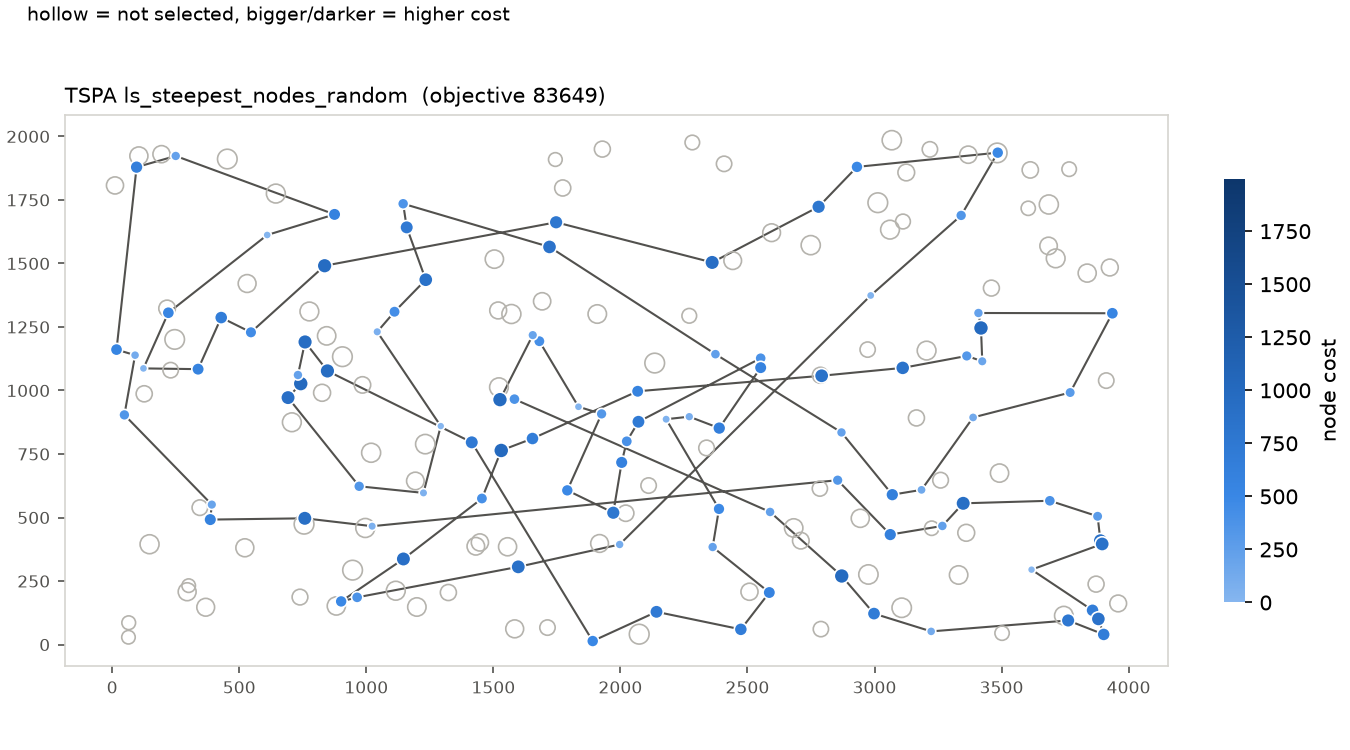
\includegraphics[width=0.85\textwidth]{plots/TSPA_ls_steepest_nodes_random.png}
  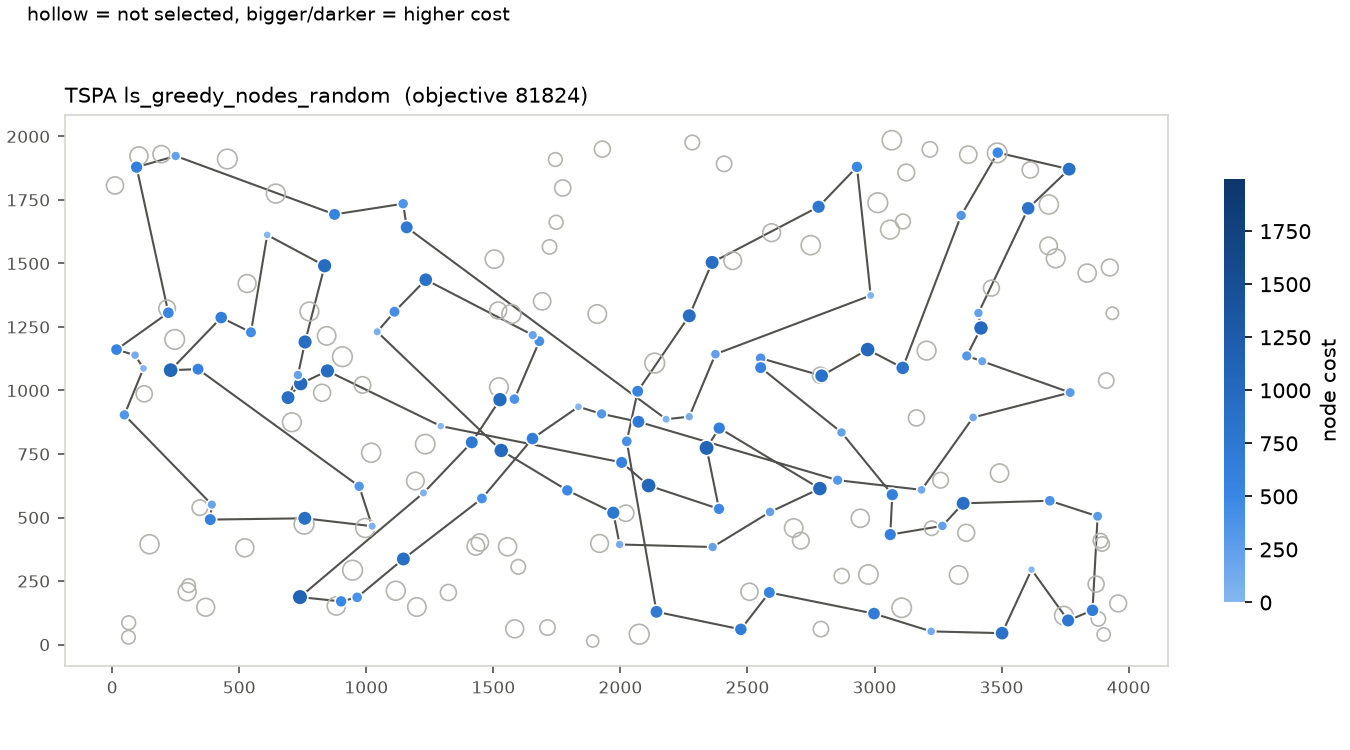
\includegraphics[width=0.85\textwidth]{plots/TSPA_ls_greedy_nodes_random.png}
\end{figure}
\begin{figure}[H]
  \centering
  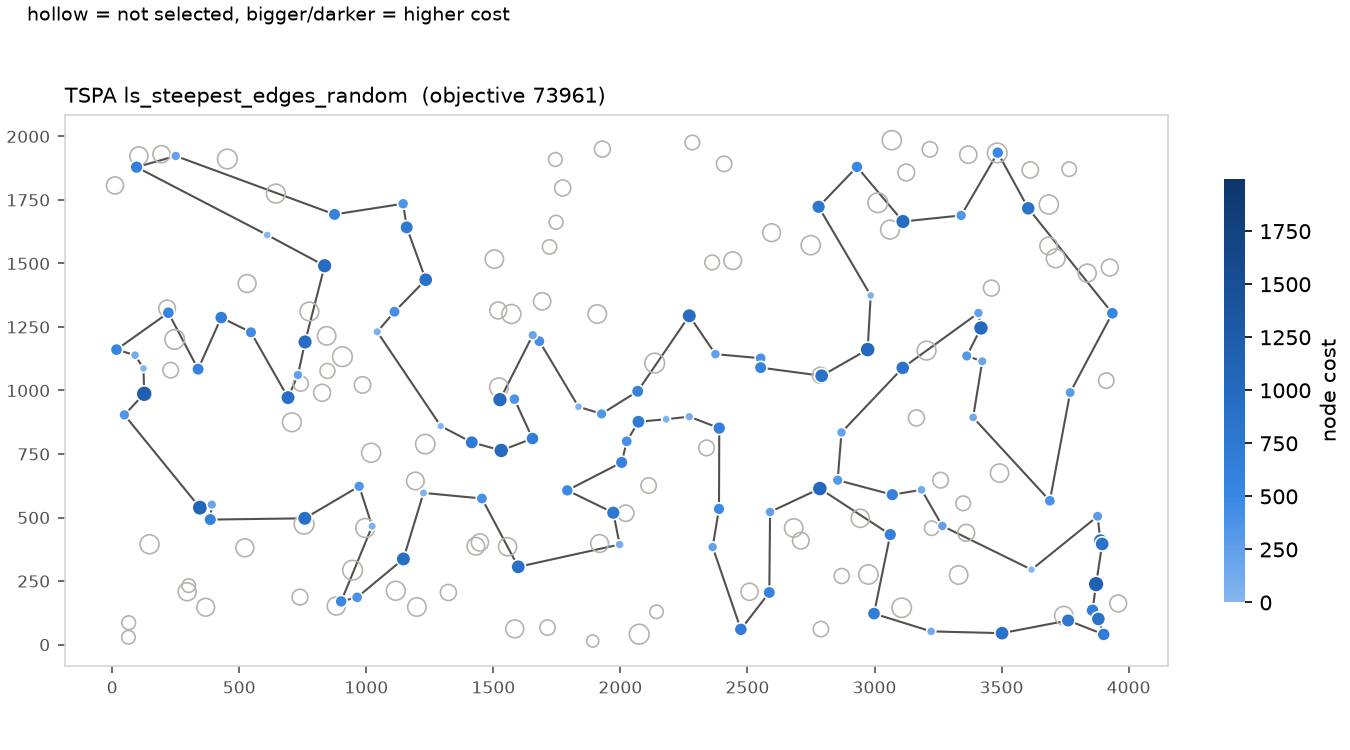
\includegraphics[width=0.85\textwidth]{plots/TSPA_ls_steepest_edges_random.png}
  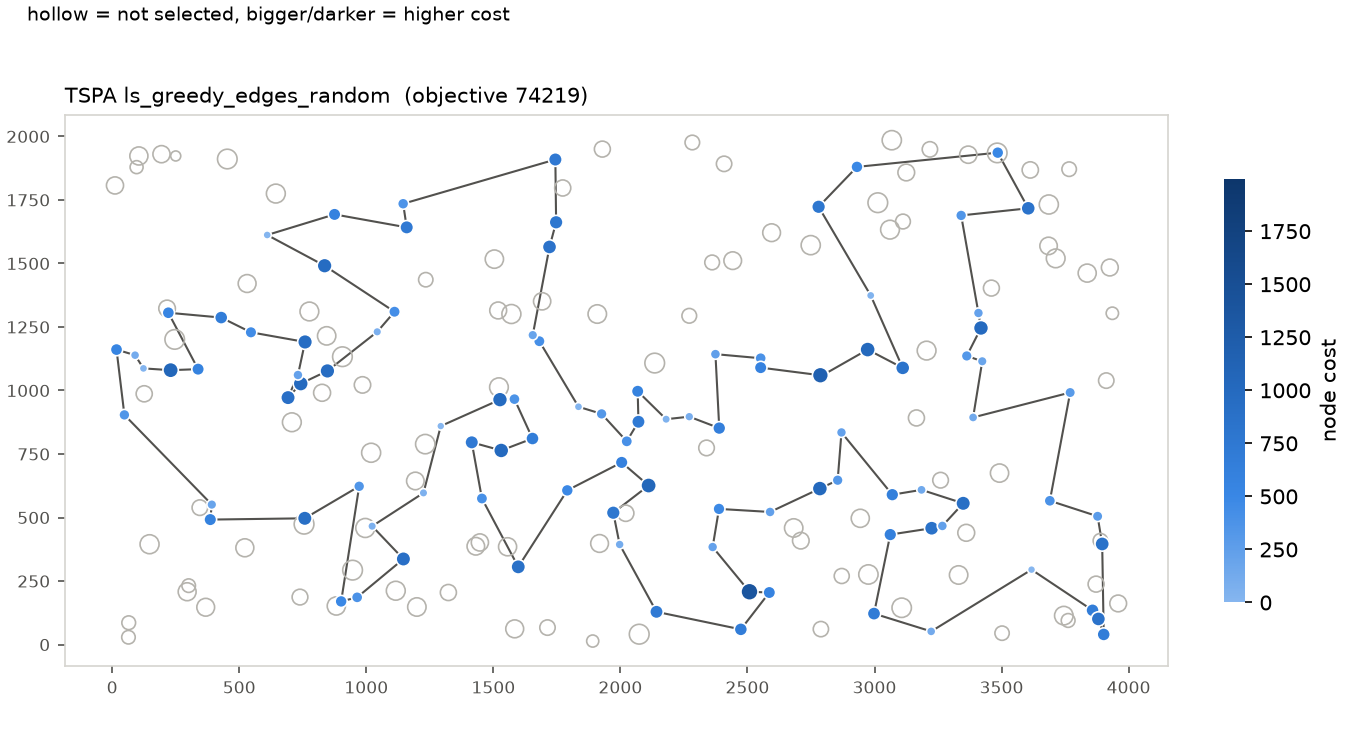
\includegraphics[width=0.85\textwidth]{plots/TSPA_ls_greedy_edges_random.png}
\end{figure}
\begin{figure}[H]
  \centering
  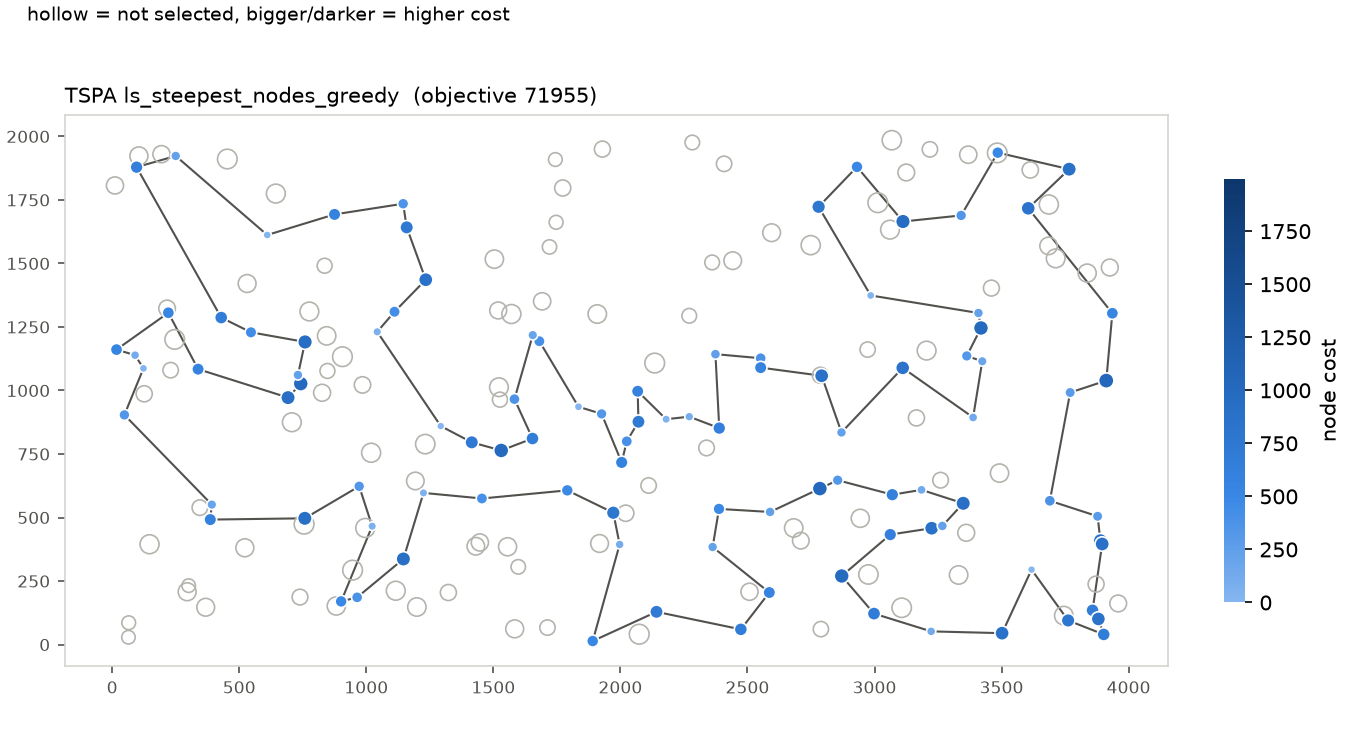
\includegraphics[width=0.85\textwidth]{plots/TSPA_ls_steepest_nodes_greedy.png}
  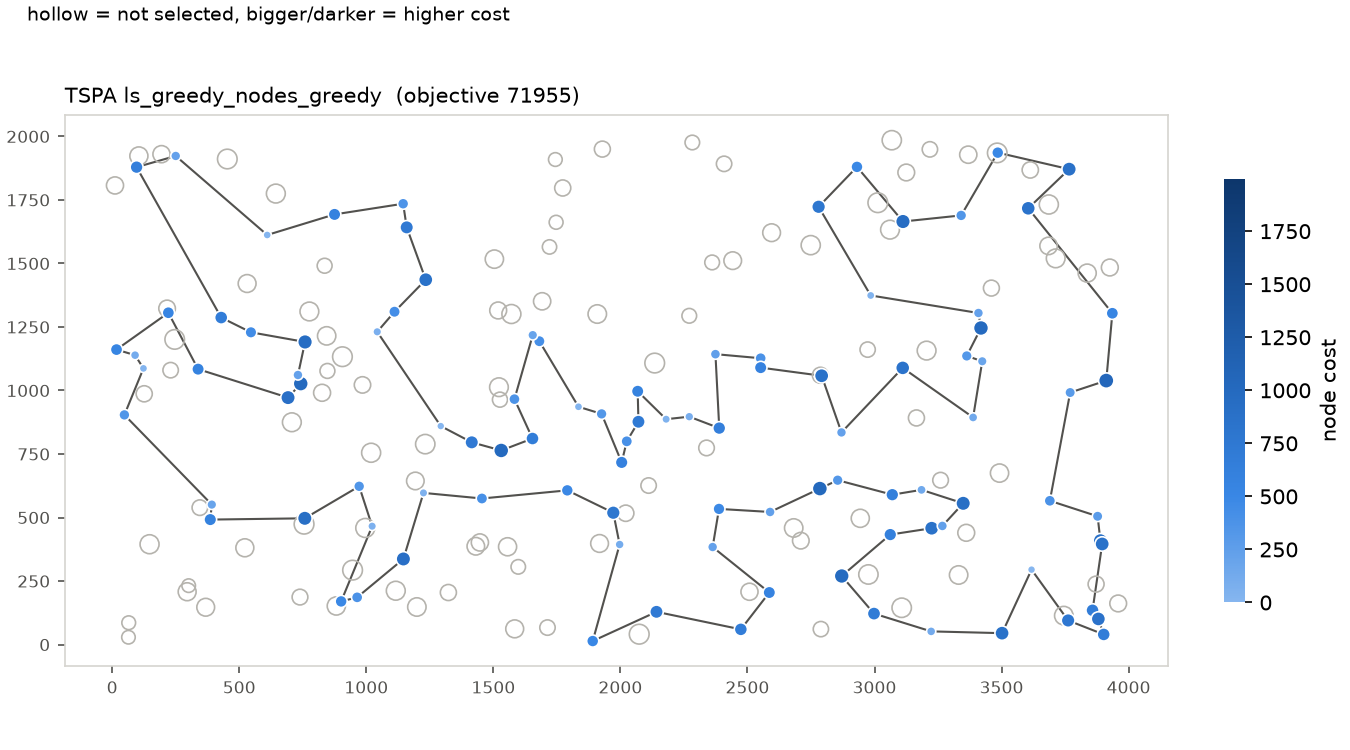
\includegraphics[width=0.85\textwidth]{plots/TSPA_ls_greedy_nodes_greedy.png}
\end{figure}
\begin{figure}[H]
  \centering
  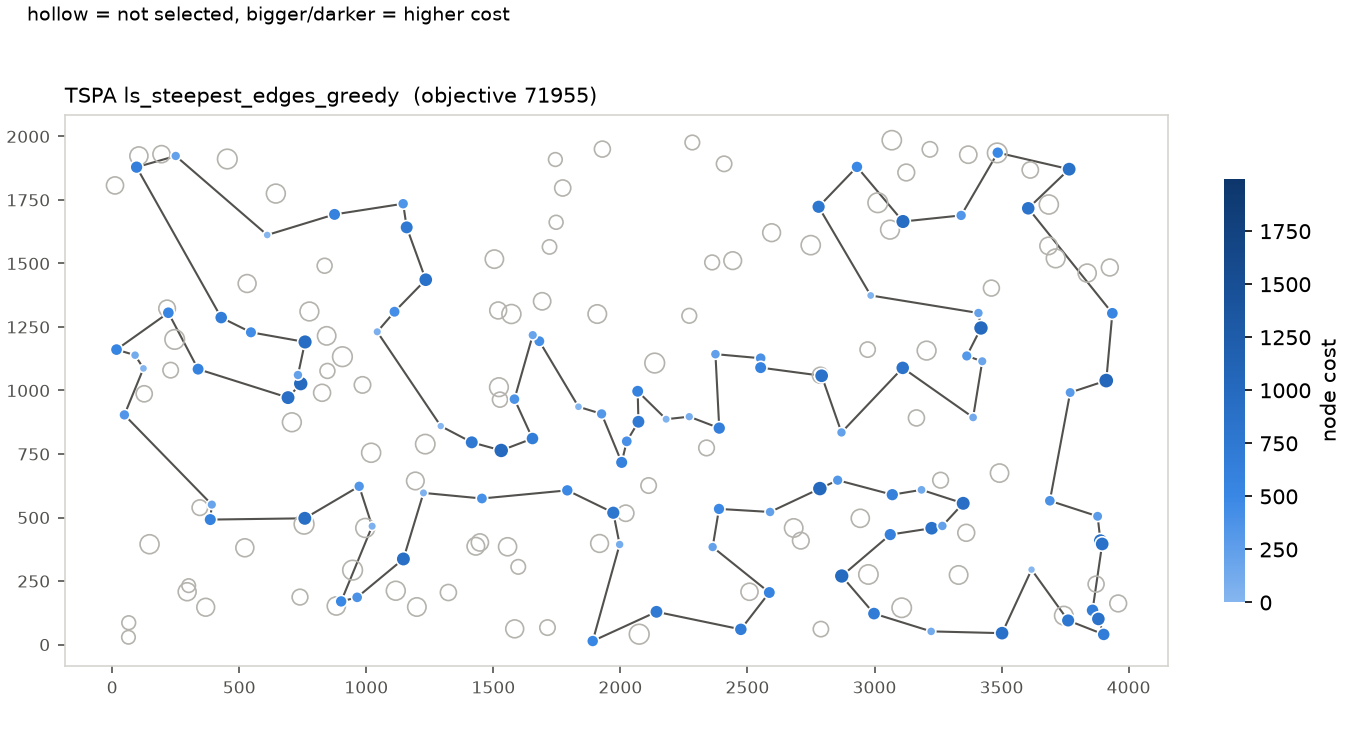
\includegraphics[width=0.85\textwidth]{plots/TSPA_ls_steepest_edges_greedy.png}
  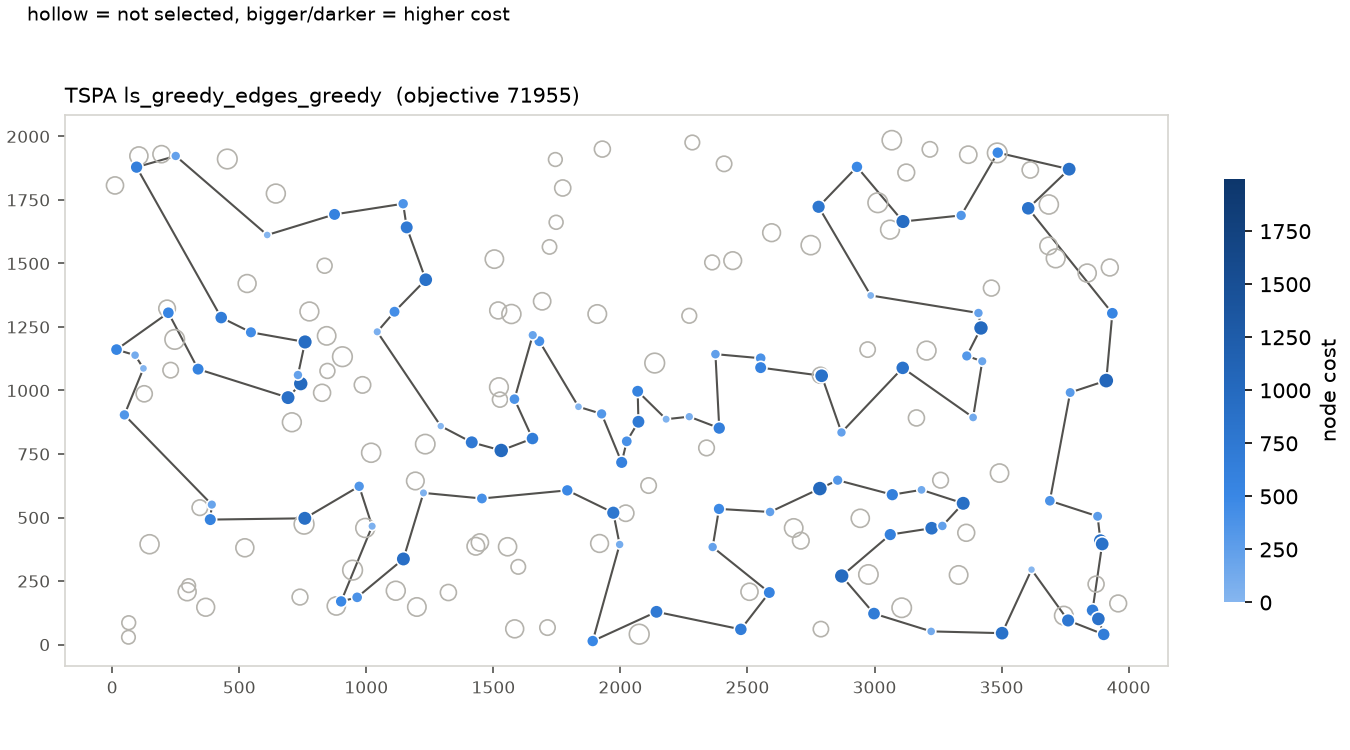
\includegraphics[width=0.85\textwidth]{plots/TSPA_ls_greedy_edges_greedy.png}
\end{figure}
\subsection*{TSPB}
\begin{figure}[H]
  \centering
  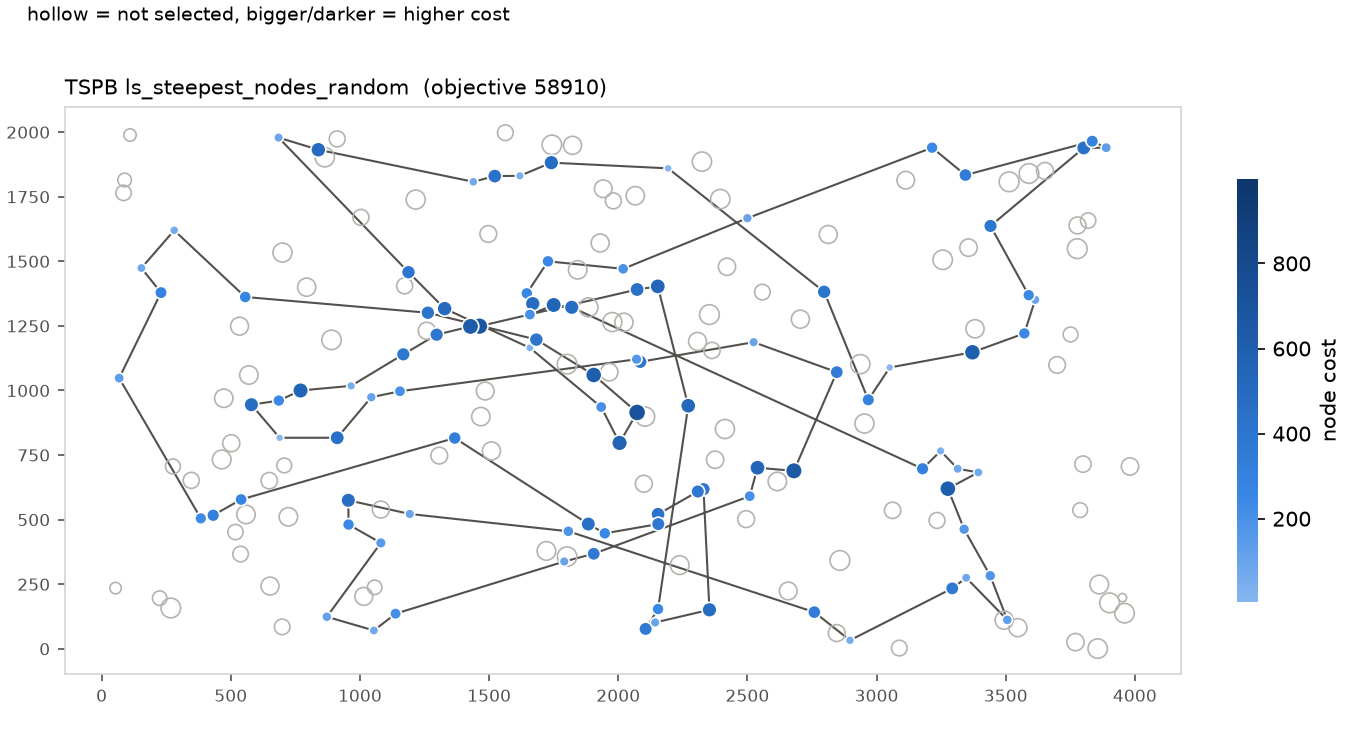
\includegraphics[width=0.85\textwidth]{plots/TSPB_ls_steepest_nodes_random.png}
  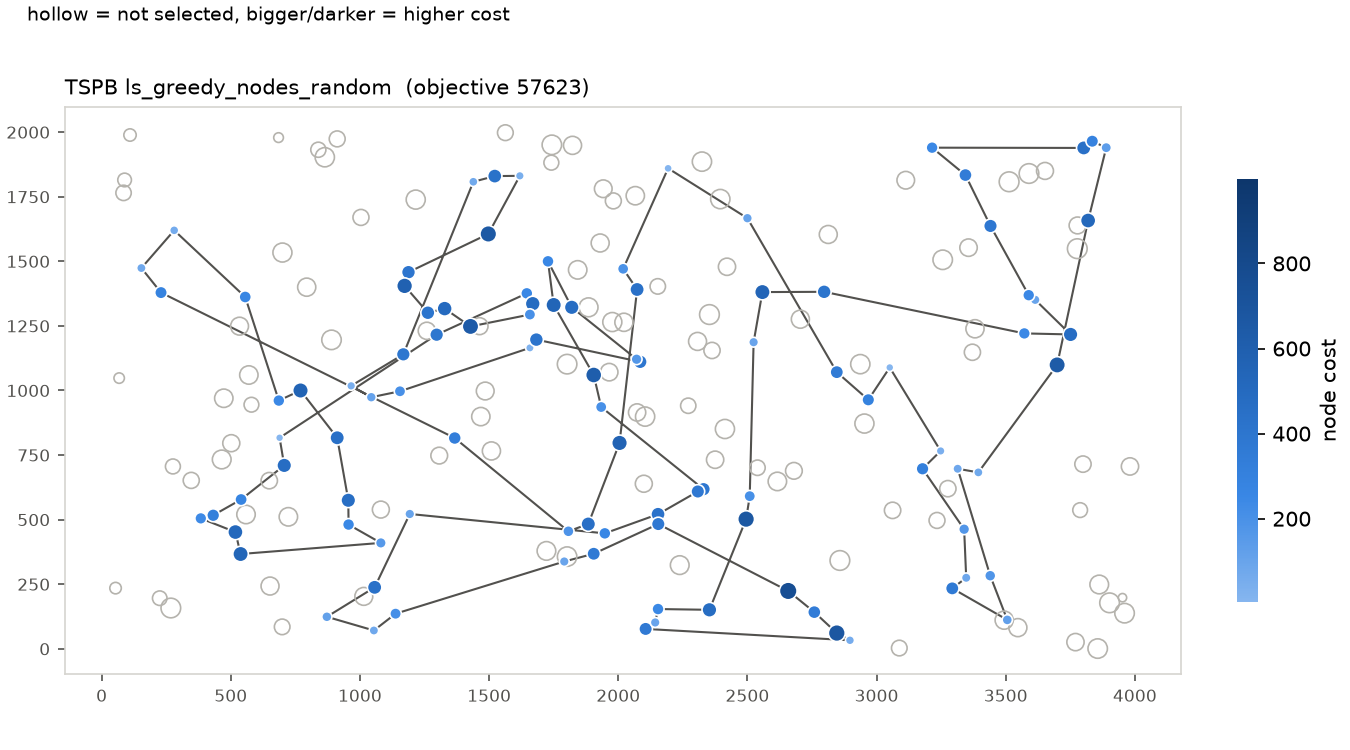
\includegraphics[width=0.85\textwidth]{plots/TSPB_ls_greedy_nodes_random.png}
\end{figure}
\begin{figure}[H]
  \centering
  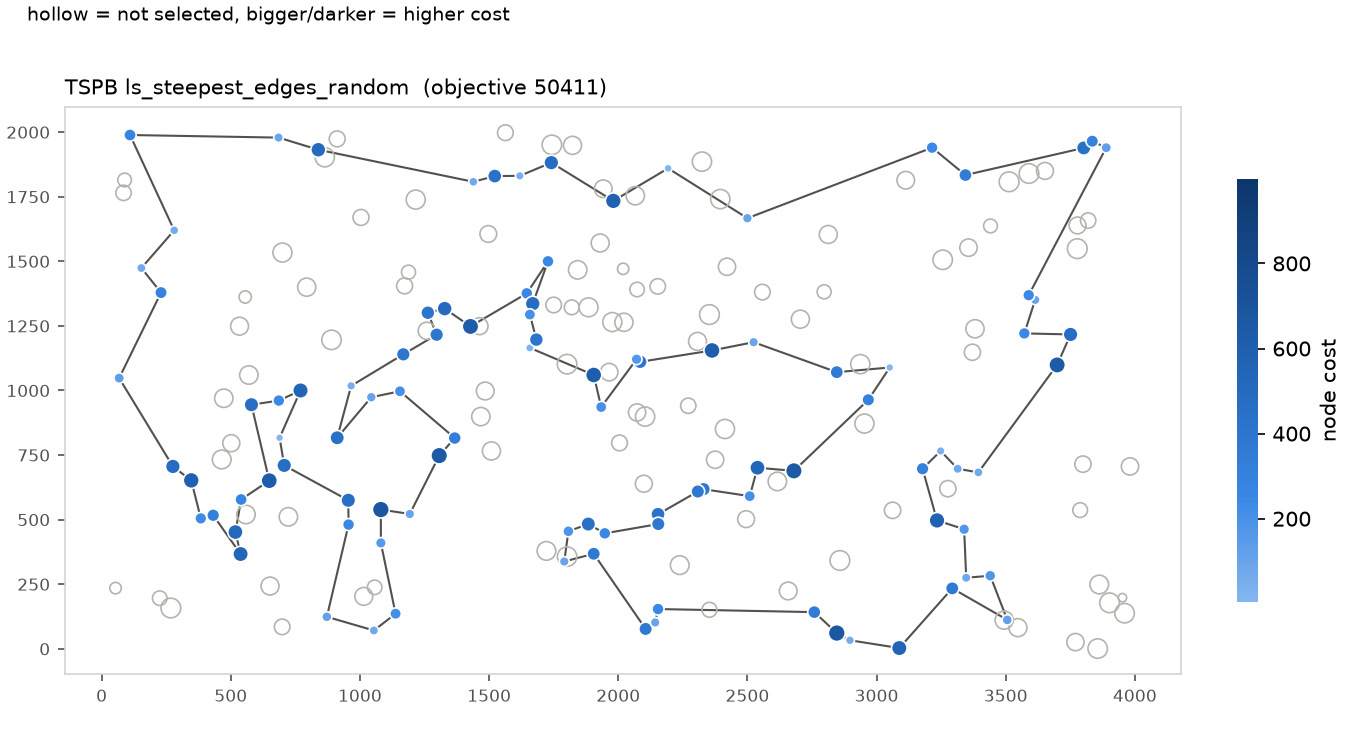
\includegraphics[width=0.85\textwidth]{plots/TSPB_ls_steepest_edges_random.png}
  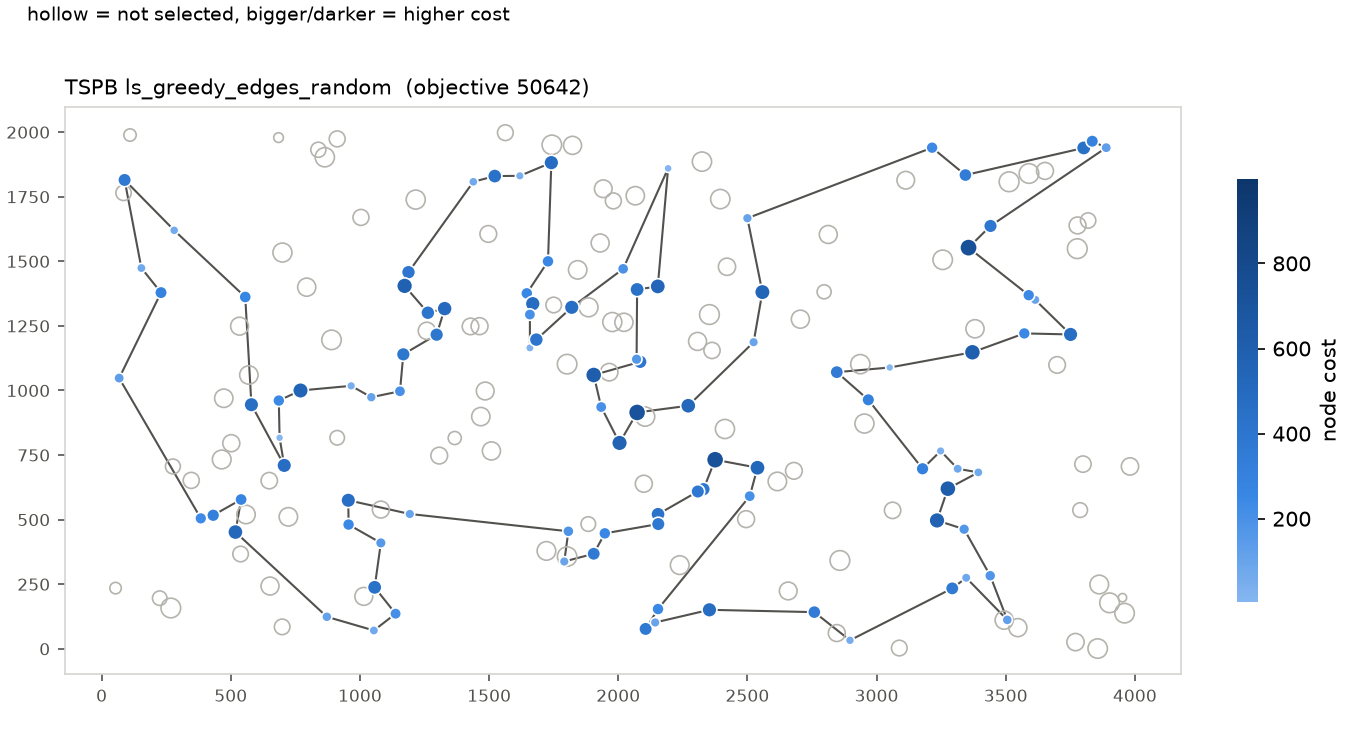
\includegraphics[width=0.85\textwidth]{plots/TSPB_ls_greedy_edges_random.png}
\end{figure}
\begin{figure}[H]
  \centering
  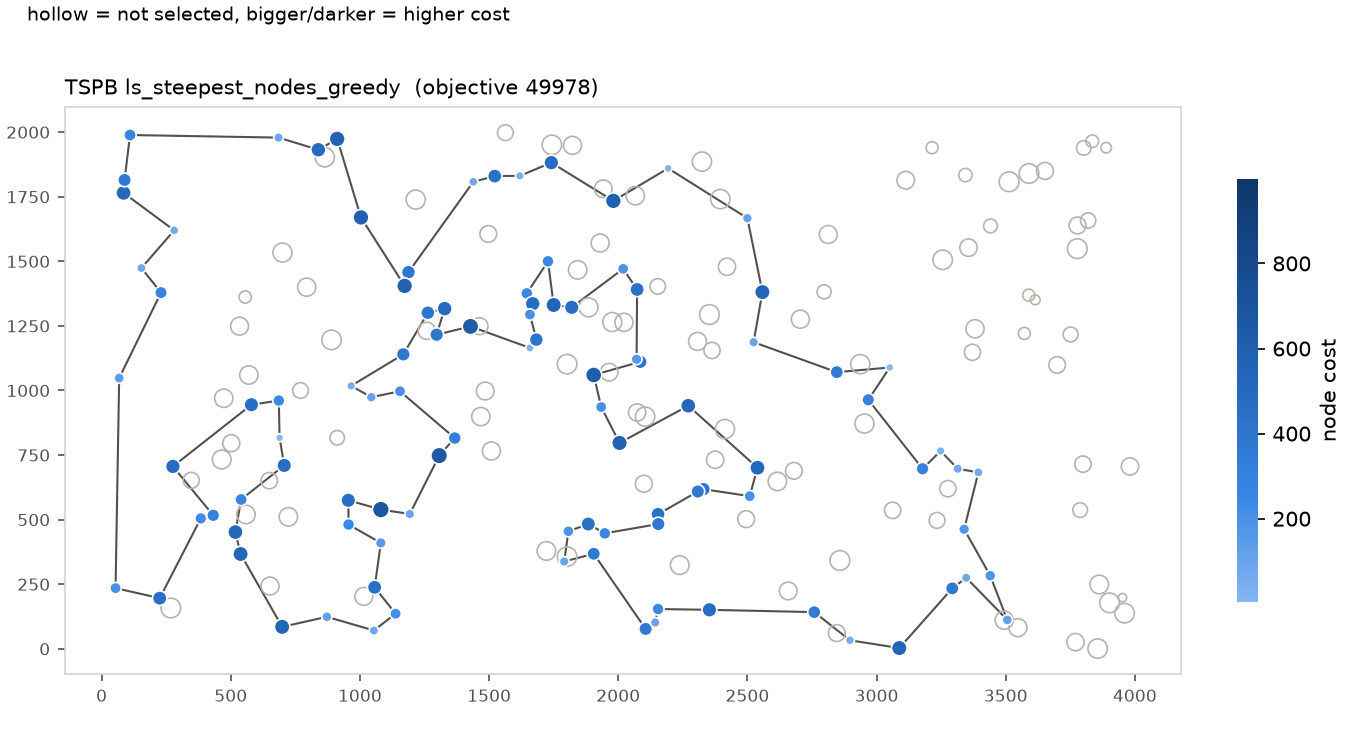
\includegraphics[width=0.85\textwidth]{plots/TSPB_ls_steepest_nodes_greedy.png}
  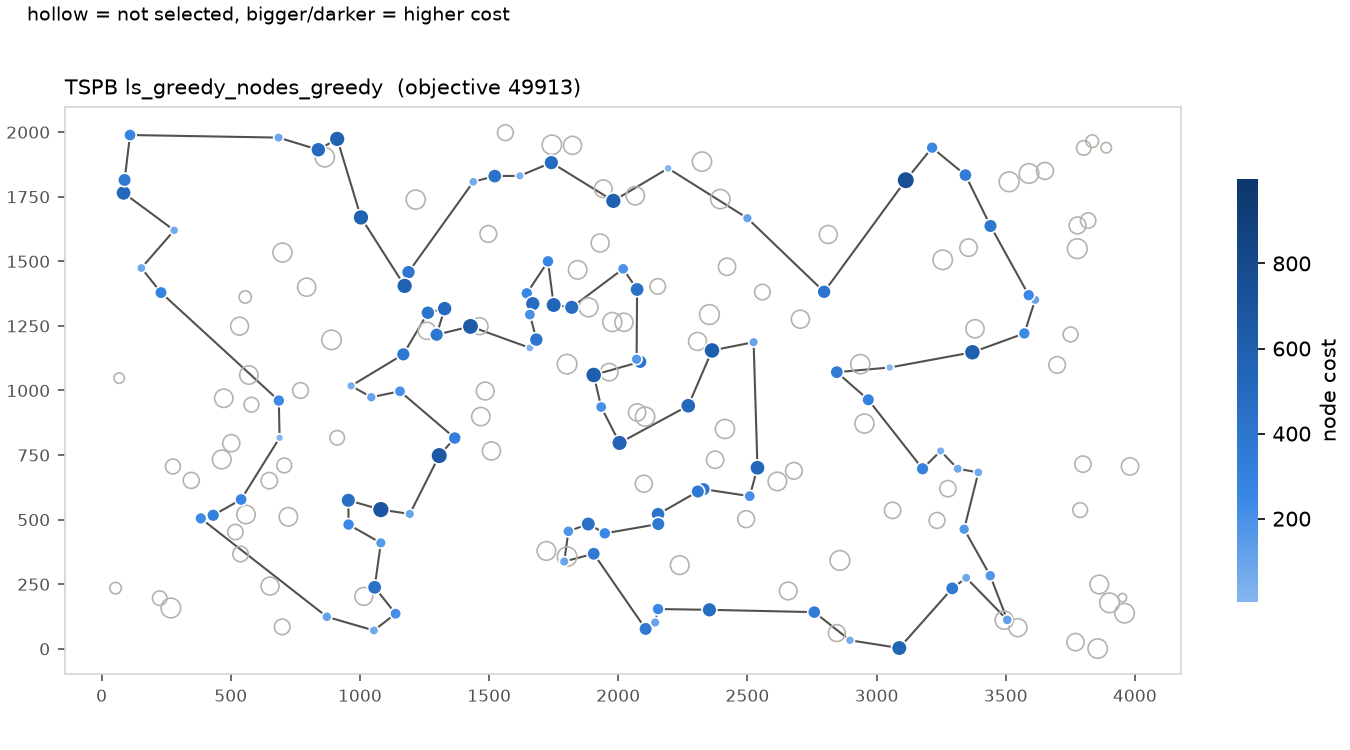
\includegraphics[width=0.85\textwidth]{plots/TSPB_ls_greedy_nodes_greedy.png}
\end{figure}
\begin{figure}[H]
  \centering
  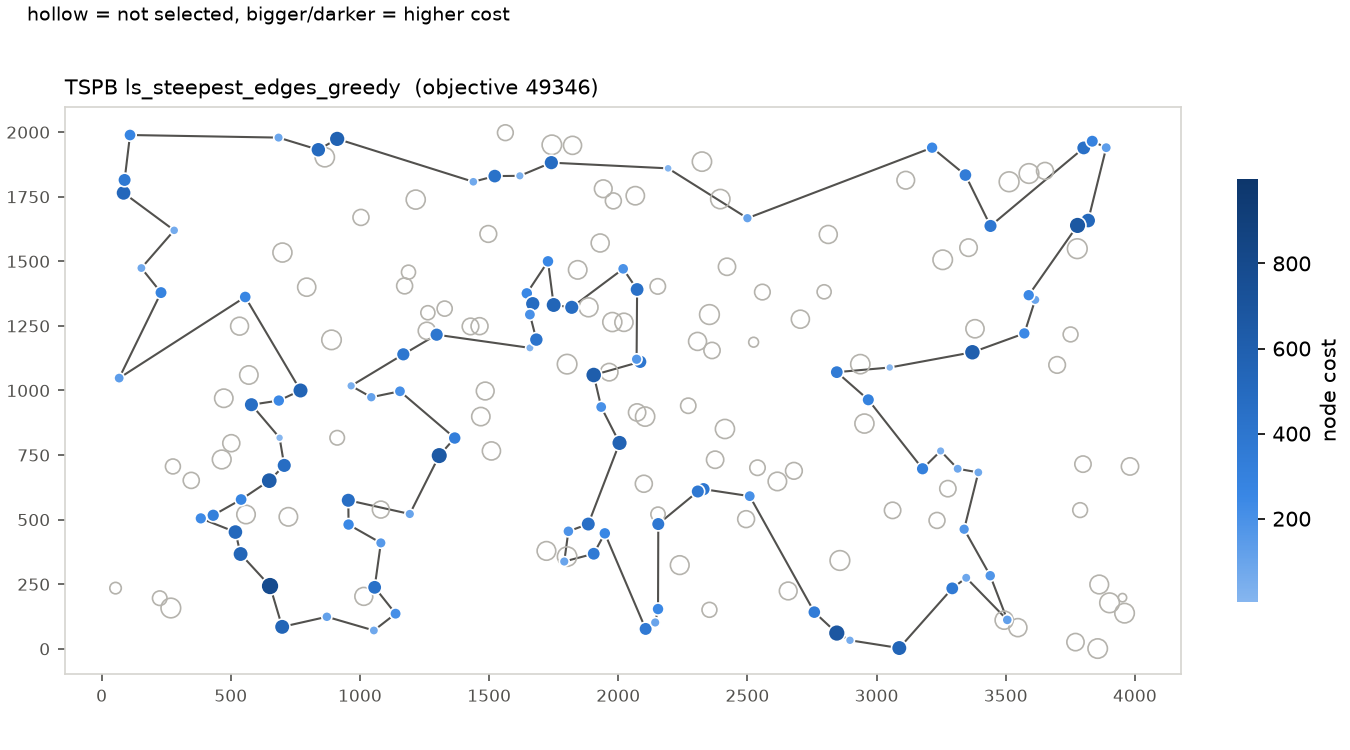
\includegraphics[width=0.85\textwidth]{plots/TSPB_ls_steepest_edges_greedy.png}
  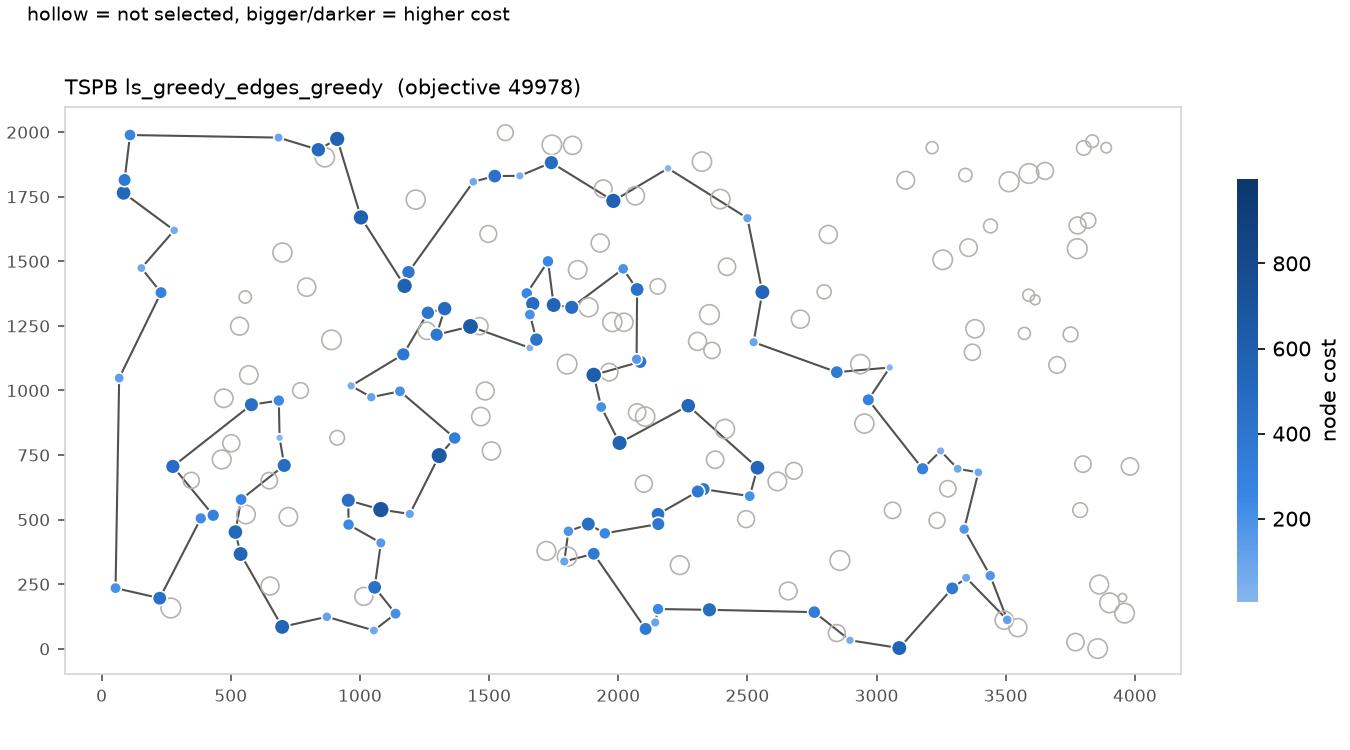
\includegraphics[width=0.85\textwidth]{plots/TSPB_ls_greedy_edges_greedy.png}
\end{figure}
% ---------------------------------------------------------------
\section{Best solutions}
Lists of node indices, starting from 0, in the order they are visited. The cycle closes from the
last node back to the first. Best solutions of the previous methods are listed in the previous
reports.
\subsection*{TSPA}

\textbf{LS steepest, two-nodes, random start} (objective 83649)
\nodelist{158, 192, 181, 114, 28, 90, 100, 123, 83, 160, 30, 141, 180, 132, 76, 4, 71, 157, 139, 33, 174, 150, 106, 93, 47, 147, 1, 169, 50, 3, 85, 8, 52, 185, 102, 87, 189, 171, 2, 98, 135, 164, 178, 29, 136, 186, 62, 112, 38, 152, 108, 49, 63, 60, 80, 91, 48, 31, 116, 149, 168, 97, 127, 161, 187, 176, 151, 89, 113, 130, 159, 146, 170, 107, 153, 193, 78, 88, 57, 182, 138, 134, 35, 156, 51, 16, 67, 144, 45, 73, 140, 53, 179, 9, 54, 131, 36, 177, 84, 58}

\textbf{LS greedy, two-nodes, random start} (objective 81824)
\nodelist{31, 60, 116, 149, 63, 168, 97, 127, 161, 187, 30, 49, 11, 108, 152, 80, 38, 100, 123, 160, 83, 90, 180, 140, 41, 84, 99, 131, 72, 134, 58, 135, 73, 45, 102, 132, 76, 4, 51, 16, 35, 156, 28, 141, 92, 171, 2, 189, 87, 185, 67, 144, 179, 176, 106, 93, 47, 50, 3, 169, 1, 101, 55, 29, 178, 85, 142, 8, 9, 54, 174, 150, 151, 89, 113, 130, 159, 153, 88, 107, 64, 57, 182, 158, 192, 181, 53, 52, 143, 62, 186, 136, 164, 33, 36, 177, 71, 157, 91, 48}

\textbf{LS steepest, two-edges, random start} (objective 73961)
\nodelist{127, 161, 30, 187, 171, 2, 189, 141, 87, 98, 135, 73, 45, 140, 53, 179, 177, 36, 131, 84, 58, 192, 158, 134, 72, 151, 182, 57, 64, 88, 78, 193, 153, 75, 170, 146, 159, 107, 89, 106, 150, 176, 174, 85, 1, 169, 3, 50, 93, 130, 47, 147, 101, 29, 178, 184, 136, 186, 164, 142, 8, 54, 9, 33, 143, 52, 144, 67, 16, 51, 156, 35, 185, 102, 28, 180, 132, 76, 4, 71, 157, 91, 48, 31, 80, 38, 100, 123, 160, 152, 108, 49, 60, 116, 149, 63, 119, 168, 95, 97}

\textbf{LS greedy, two-edges, random start} (objective 74219)
\nodelist{189, 187, 141, 180, 156, 35, 185, 102, 28, 87, 98, 45, 140, 41, 73, 135, 181, 192, 158, 20, 58, 84, 134, 72, 176, 174, 150, 106, 113, 89, 42, 151, 182, 57, 107, 153, 193, 78, 170, 159, 130, 47, 93, 50, 3, 169, 1, 178, 101, 29, 136, 186, 164, 85, 142, 8, 194, 54, 9, 33, 131, 36, 177, 52, 179, 53, 144, 67, 16, 51, 139, 112, 115, 157, 71, 91, 80, 38, 76, 132, 90, 83, 160, 123, 100, 152, 108, 60, 49, 11, 63, 149, 116, 168, 97, 127, 161, 30, 171, 2}

\textbf{LS steepest, two-nodes, greedy start} (objective 71955)
\nodelist{55, 29, 178, 184, 136, 186, 164, 1, 169, 3, 50, 93, 85, 174, 8, 54, 9, 33, 131, 36, 177, 52, 179, 53, 140, 144, 67, 16, 51, 35, 185, 102, 28, 180, 132, 76, 4, 71, 157, 91, 80, 48, 31, 108, 152, 100, 123, 83, 160, 49, 60, 116, 149, 63, 168, 97, 127, 161, 30, 187, 171, 2, 189, 141, 87, 45, 73, 135, 114, 181, 192, 158, 58, 84, 134, 72, 176, 150, 106, 113, 89, 42, 151, 138, 182, 57, 64, 107, 88, 78, 193, 153, 170, 146, 159, 130, 47, 37, 147, 101}

\textbf{LS greedy, two-nodes, greedy start} (objective 71955)
\nodelist{55, 29, 178, 184, 136, 186, 164, 1, 169, 3, 50, 93, 85, 174, 8, 54, 9, 33, 131, 36, 177, 52, 179, 53, 140, 144, 67, 16, 51, 35, 185, 102, 28, 180, 132, 76, 4, 71, 157, 91, 80, 48, 31, 108, 152, 100, 123, 83, 160, 49, 60, 116, 149, 63, 168, 97, 127, 161, 30, 187, 171, 2, 189, 141, 87, 45, 73, 135, 114, 181, 192, 158, 58, 84, 134, 72, 176, 150, 106, 113, 89, 42, 151, 138, 182, 57, 64, 107, 88, 78, 193, 153, 170, 146, 159, 130, 47, 37, 147, 101}

\textbf{LS steepest, two-edges, greedy start} (objective 71955)
\nodelist{101, 147, 37, 47, 130, 159, 146, 170, 153, 193, 78, 88, 107, 64, 57, 182, 138, 151, 42, 89, 113, 106, 150, 176, 72, 134, 84, 58, 158, 192, 181, 114, 135, 73, 45, 87, 141, 189, 2, 171, 187, 30, 161, 127, 97, 168, 63, 149, 116, 60, 49, 160, 83, 123, 100, 152, 108, 31, 48, 80, 91, 157, 71, 4, 76, 132, 180, 28, 102, 185, 35, 51, 16, 67, 144, 140, 53, 179, 52, 177, 36, 131, 33, 9, 54, 8, 174, 85, 93, 50, 3, 169, 1, 164, 186, 136, 184, 178, 29, 55}

\textbf{LS greedy, two-edges, greedy start} (objective 71955)
\nodelist{101, 147, 37, 47, 130, 159, 146, 170, 153, 193, 78, 88, 107, 64, 57, 182, 138, 151, 42, 89, 113, 106, 150, 176, 72, 134, 84, 58, 158, 192, 181, 114, 135, 73, 45, 87, 141, 189, 2, 171, 187, 30, 161, 127, 97, 168, 63, 149, 116, 60, 49, 160, 83, 123, 100, 152, 108, 31, 48, 80, 91, 157, 71, 4, 76, 132, 180, 28, 102, 185, 35, 51, 16, 67, 144, 140, 53, 179, 52, 177, 36, 131, 33, 9, 54, 8, 174, 85, 93, 50, 3, 169, 1, 164, 186, 136, 184, 178, 29, 55}
\subsection*{TSPB}

\textbf{LS steepest, two-nodes, random start} (objective 58910)
\nodelist{99, 59, 40, 155, 71, 60, 175, 134, 45, 85, 51, 67, 66, 84, 162, 76, 3, 184, 47, 140, 97, 170, 177, 125, 26, 154, 38, 21, 189, 168, 46, 86, 27, 179, 82, 87, 88, 24, 34, 152, 181, 167, 73, 64, 6, 29, 132, 65, 145, 28, 149, 158, 30, 160, 122, 111, 98, 151, 69, 183, 130, 116, 147, 121, 198, 96, 48, 89, 104, 192, 54, 78, 10, 114, 196, 187, 81, 105, 94, 70, 190, 57, 72, 120, 133, 136, 172, 8, 117, 80, 127, 129, 90, 52, 153, 14, 2, 20, 74, 171}

\textbf{LS greedy, two-nodes, random start} (objective 57623)
\nodelist{71, 60, 36, 197, 132, 29, 6, 115, 170, 21, 133, 136, 172, 189, 183, 30, 191, 130, 63, 96, 198, 121, 38, 154, 140, 47, 69, 160, 3, 184, 117, 120, 8, 122, 151, 24, 34, 152, 167, 40, 157, 175, 134, 45, 85, 51, 181, 163, 99, 39, 171, 82, 87, 179, 88, 31, 67, 76, 185, 104, 10, 148, 114, 196, 187, 70, 190, 81, 94, 105, 61, 143, 90, 129, 14, 2, 74, 20, 153, 80, 127, 54, 192, 162, 57, 89, 72, 46, 98, 73, 59, 64, 145, 28, 149, 158, 125, 26, 97, 155}

\textbf{LS steepest, two-edges, random start} (objective 50411)
\nodelist{197, 36, 29, 132, 103, 178, 65, 145, 28, 149, 37, 116, 147, 121, 198, 96, 48, 156, 89, 57, 190, 70, 81, 94, 105, 196, 114, 10, 148, 143, 90, 129, 127, 80, 182, 153, 20, 14, 2, 74, 17, 171, 39, 99, 179, 87, 82, 51, 85, 59, 73, 167, 181, 152, 34, 24, 67, 66, 84, 192, 54, 162, 76, 135, 3, 184, 151, 122, 69, 160, 172, 136, 120, 133, 189, 183, 30, 21, 38, 154, 97, 140, 47, 64, 33, 40, 141, 60, 45, 134, 175, 71, 155, 115, 170, 26, 125, 177, 180, 6}

\textbf{LS greedy, two-edges, random start} (objective 50642)
\nodelist{127, 80, 192, 162, 54, 78, 10, 148, 114, 196, 18, 187, 105, 94, 81, 70, 190, 57, 185, 76, 27, 111, 98, 151, 122, 3, 184, 46, 86, 89, 72, 117, 160, 69, 172, 136, 133, 120, 48, 96, 198, 121, 130, 191, 30, 183, 21, 38, 47, 140, 154, 26, 125, 170, 115, 177, 158, 149, 146, 28, 145, 65, 132, 29, 6, 197, 175, 134, 45, 157, 60, 71, 155, 40, 59, 85, 51, 167, 181, 152, 34, 24, 11, 66, 67, 179, 82, 87, 88, 99, 171, 74, 20, 2, 14, 153, 182, 52, 90, 129}

\textbf{LS steepest, two-nodes, greedy start} (objective 49978)
\nodelist{65, 145, 28, 149, 13, 146, 37, 116, 147, 42, 50, 191, 130, 121, 198, 96, 48, 156, 89, 57, 185, 76, 162, 54, 192, 80, 127, 129, 90, 153, 14, 2, 20, 74, 17, 171, 99, 88, 179, 87, 82, 51, 85, 59, 73, 167, 181, 152, 34, 24, 67, 66, 27, 98, 151, 122, 3, 184, 46, 72, 117, 8, 120, 133, 136, 172, 160, 69, 189, 21, 183, 30, 38, 154, 140, 47, 64, 33, 40, 141, 155, 71, 60, 157, 45, 134, 175, 62, 36, 197, 6, 115, 170, 125, 177, 178, 29, 132, 174, 1}

\textbf{LS greedy, two-nodes, greedy start} (objective 49913)
\nodelist{125, 145, 28, 149, 13, 146, 37, 116, 147, 42, 50, 191, 130, 121, 198, 96, 48, 156, 89, 57, 104, 194, 190, 70, 187, 196, 114, 10, 78, 54, 162, 192, 80, 127, 129, 90, 153, 14, 2, 20, 74, 17, 171, 99, 88, 179, 87, 82, 51, 85, 59, 73, 167, 181, 152, 34, 24, 67, 66, 76, 135, 27, 98, 151, 122, 3, 184, 46, 72, 117, 8, 120, 133, 136, 172, 160, 69, 189, 21, 183, 30, 38, 154, 140, 47, 64, 33, 40, 141, 155, 71, 60, 157, 45, 134, 175, 132, 29, 6, 170}

\textbf{LS steepest, two-edges, greedy start} (objective 49346)
\nodelist{65, 145, 28, 149, 13, 146, 37, 116, 147, 42, 121, 198, 96, 48, 89, 57, 190, 70, 187, 81, 94, 105, 61, 139, 196, 114, 10, 78, 54, 162, 192, 80, 127, 129, 90, 153, 14, 2, 20, 74, 17, 171, 39, 99, 67, 24, 34, 181, 179, 87, 82, 167, 51, 85, 59, 73, 98, 151, 122, 3, 184, 46, 72, 117, 8, 120, 133, 136, 172, 160, 69, 21, 38, 154, 140, 47, 64, 33, 40, 155, 71, 60, 157, 45, 134, 175, 62, 91, 36, 197, 132, 29, 6, 180, 115, 170, 177, 125, 26, 158}

\textbf{LS greedy, two-edges, greedy start} (objective 49978)
\nodelist{65, 145, 28, 149, 13, 146, 37, 116, 147, 42, 50, 191, 130, 121, 198, 96, 48, 156, 89, 57, 185, 76, 162, 54, 192, 80, 127, 129, 90, 153, 14, 2, 20, 74, 17, 171, 99, 88, 179, 87, 82, 51, 85, 59, 73, 167, 181, 152, 34, 24, 67, 66, 27, 98, 151, 122, 3, 184, 46, 72, 117, 8, 120, 133, 136, 172, 160, 69, 189, 21, 183, 30, 38, 154, 140, 47, 64, 33, 40, 141, 155, 71, 60, 157, 45, 134, 175, 62, 36, 197, 6, 115, 170, 125, 177, 178, 29, 132, 174, 1}
% ---------------------------------------------------------------
\section{Solution checker}
All sixteen best solutions of the local search methods were checked with the provided solution
checker (\texttt{Solution checker.xlsx}), and every objective value matches. Our code additionally
checks every generated solution for the number of nodes and for repeated nodes.
\begin{table}[H]
\centering
\small
\begin{tabular}{llrrc}
\toprule
Instance & Method & Our objective & Checker objective & Match \\
\midrule
TSPA & LS steepest, two-nodes, random start & 83649 & 83649 & yes \\
TSPA & LS greedy, two-nodes, random start & 81824 & 81824 & yes \\
TSPA & LS steepest, two-edges, random start & 73961 & 73961 & yes \\
TSPA & LS greedy, two-edges, random start & 74219 & 74219 & yes \\
TSPA & LS steepest, two-nodes, greedy start & 71955 & 71955 & yes \\
TSPA & LS greedy, two-nodes, greedy start & 71955 & 71955 & yes \\
TSPA & LS steepest, two-edges, greedy start & 71955 & 71955 & yes \\
TSPA & LS greedy, two-edges, greedy start & 71955 & 71955 & yes \\
\midrule
TSPB & LS steepest, two-nodes, random start & 58910 & 58910 & yes \\
TSPB & LS greedy, two-nodes, random start & 57623 & 57623 & yes \\
TSPB & LS steepest, two-edges, random start & 50411 & 50411 & yes \\
TSPB & LS greedy, two-edges, random start & 50642 & 50642 & yes \\
TSPB & LS steepest, two-nodes, greedy start & 49978 & 49978 & yes \\
TSPB & LS greedy, two-nodes, greedy start & 49913 & 49913 & yes \\
TSPB & LS steepest, two-edges, greedy start & 49346 & 49346 & yes \\
TSPB & LS greedy, two-edges, greedy start & 49978 & 49978 & yes \\
\bottomrule
\end{tabular}
\end{table}

% ---------------------------------------------------------------
\section{Conclusions}

\begin{itemize}
  \item The two-edges exchange is a much better intra-route move than the two-nodes exchange. From
        random starts it gives 76\,185 vs.\ 90\,367 on TSPA and 52\,685 vs.\ 65\,818 on TSPB (steepest
        version). A two-edges exchange removes a crossing of two edges in one move, while
        swapping two nodes changes four edges at once and usually makes the tour longer, so the
        local optima of the two-nodes neighborhood still contain many crossings and detours.
  \item Local search improves every starting solution, and the starting solution matters a lot.
        On TSPA the greedy starts give the best results (72\,976 on average, best 71\,955, vs.\
        73\,353.5 for the greedy heuristic alone). On TSPB the steepest two-edges search from
        random starts has the best average (52\,685.1), slightly better than from greedy starts
        (53\,092.0), but the best single solution comes from a greedy start (49\,346). The best
        solutions of both instances are now better than all solutions of the previous methods
        (TSPA 71\,955 vs.\ 72\,011, TSPB 49\,346 vs.\ 50\,485).
  \item On TSPA the greedy solutions are already almost local optima: local search applies only 3--5
        moves, the average improves by only 0.5\%, and all four greedy-start methods give the same
        minimum and maximum. On TSPB the greedy solutions are further from a local optimum
        (10--26 moves) and local search improves the average by 2.5\% (two-nodes) to 4.7\%
        (two-edges).
  \item Steepest and greedy local search give results of very similar quality, the differences are
        at most 0.6\%. The only clear difference is the two-nodes neighborhood from random
        starts, where greedy is about 2.3--3.5\% better than steepest.
  \item Greedy local search needs about 3 times more iterations (about 420 vs.\ 130--150 from
        random starts), because it applies the first improving move instead of the best one, but it
        evaluates 16--21 times fewer moves (95--142 thousand vs.\ 2.0--2.3 million).
  \item Thanks to that, greedy local search is about 5 times faster than steepest from random starts
        (129--172\,ms vs.\ 680--935\,ms). The speed-up is smaller than the reduction of evaluated
        moves, because one move is more expensive in greedy (about 1.2--1.4\,$\mu$s vs.\
        0.35--0.4\,$\mu$s): every iteration draws a new random permutation of all moves, which is
        a large part of the time when the first improving move is found quickly.
  \item Local search from greedy starts is much faster (26--102\,ms), because only a few moves are
        needed. Here greedy is 1.2--1.3 times faster than steepest on TSPA, where steepest needs only
        3--4 iterations, and about 2.3 times faster on TSPB. The construction of the greedy start
        itself takes about 64\,ms, which is not included in the local search time.
  \item The two-edges neighborhood is also faster than the two-nodes one from random starts:
        the local optimum is reached in fewer iterations (133 vs.\ 150--153 for steepest), and a
        two-edges delta is cheaper to compute (4 edges instead of 8).
\end{itemize}

\end{document}
